
\section{Création de \\ Personnage}
\lettrine{L}{e} c\oe{}ur des jeux de rôle réside dans la possibilité de créer, améliorer et faire évoluer son propre personnage. Voilà comment ça fonctionne dans {\jedifont \doctitle}. 

\subsection{Les Attributs}
Chaque personnage commence le jeu avec d4 dans chaque Attribut et dispose de 5pt pour les améliorer. Améliorer l'un d'entre eux d’un type de dé (par exemple, de d4 à d6) coûte 1 point avec une limite : vous ne pouvez aller au-delà du d12.

\subsection{Compétences}
Les Compétences représentent les aptitudes apprises comme le Tir, le Combat, les connaissances professionnelles ou scientifiques et ainsi de suite. Elles sont générales et englobent tous les aspects qui leur sont reliés. Par exemple Tir englobe les fusils, les arcs, les lance-roquettes et toutes les armes à distance. Vous disposez de 15 points à répartir entre vos Compétences. Chaque dé de Compétence coûte 1 point (en commençant à d4) tant qu’il est inférieur ou égal à l’Attribut dont il dépend (noté entre parenthèses près du nom de la Compétence). Chaque dé de Compétence supérieur à l’Attribut dont il dépend coûte 2 points. De même que pour les Attributs, aucune Compétence ne peut dépasser d12.

\subsection{Atouts & Handicaps}
Faire naître un héro digne de ce nom ne se limite pas à lui faire grimper ses attributs et ses compétences. Ce qui fait la singularité d'un héro et qui le rend fun à jouer c'est ses Atouts et ses Handicaps. De la blonde très séduisante au Jedi Agè, vous prendrez toujours plus de plaisir à jouer un personnage unique dans ses détails que le jeune humain sans problème que vous êtes tout les jours.

Vous pouvez choisir jusqu’à 1 Handicap Majeur et 2 Handicaps Mineurs. Un Handicap Majeur donne 2 points et un Handicap Mineur 1 point.

Pour 2 points vous pouvez :
\begin{itemize}
    \item Augmenter un Attribut d’un type de dé (vous pouvez le faire avant de prendre vos Compétences).
    \item Choisir un Atout.
\end{itemize}

Pour 1 point vous pouvez :
\begin{itemize}
    \item Gagner un point de Compétence.
    \item Doubler vos fonds de départ (si vous débutez avec 500\$ vous obtenez 500\$ de plus).
\end{itemize}

\subsection{Races Jouables}
% To be balanced correctly, all races most have CAP +2
Vous pouvez choisir pour votre personnage n’importe quelle race disponible dans l'univers de Star Wars. L'orientation de chaque race est donnée à titre indicatif, chaque race possède des exceptions parmis ses héros.

\subsubsection{Humain}
\begin{samepage}
	\begin{flushright}
		\begin{tabular}{ l l }
			\textbf{Type} 			& Humanoïde \\
		   	\textbf{Planète} 		& Terre \\
		   	\textbf{Langage} 		& Basic \\
		   	\textbf{Orientation} 	& Neutre \\
		\end{tabular}
	\end{flushright}

	\vspace{-6\baselineskip}
	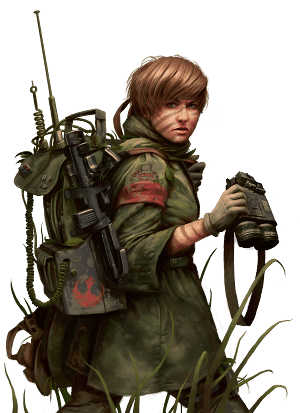
\includegraphics[width=5cm]{img/personnages/races/humain.png} 
\end{samepage}

Cette race comprend aussi bien les humains au sens strict (qu’ils soient originaires de Coruscant, de Correlia, de Kuat, de Naboo\ldots) que les humanoïdes dont les caractéristiques physiques, intellectuelles, sociales et culturelles sont suffisamment proches de celles des humains pour qu’il soit possible de les assimiler en termes de jeu.

\begin{description}[align=left]
\item [Adaptabilité] 	%CAP +2
	Les humains sont une race pleine de ressources, ils s’adaptent rapidement à toutes sorte de difficultés ou environnements.\\
	\emph{Compétence à d6}
\end{description}
\subsubsection{Barabel}
\begin{samepage}
	\begin{flushright}
		\begin{tabular}{ l l }
			\textbf{Type} 			& Reptile \\
		   	\textbf{Planète} 		& Barab I \\
		   	\textbf{Langage} 		& Barabel \\
		   	\textbf{Orientation} 	& Obscur \\
		\end{tabular}
	\end{flushright}

	\vspace{-5\baselineskip}
	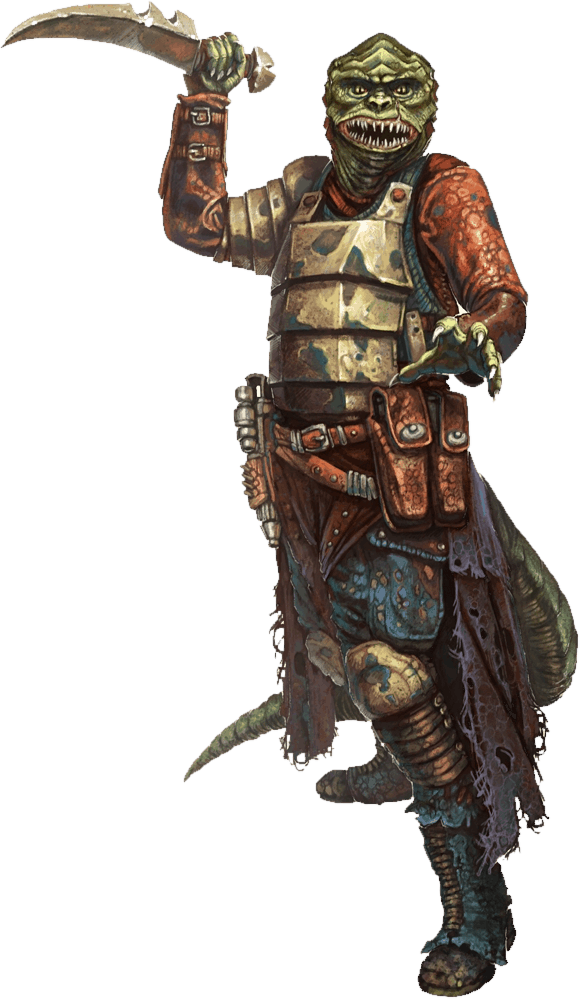
\includegraphics[width=5cm]{img/personnages/races/barabel.png}
\end{samepage}

Originaire de Barab I, les Barabels sont resté une race relativement primitive et isolée. Les Barabels vivent en clans dans un société principalement matriarcale. Ils sont fasciné par la guerre, la violence et les armes. Les Barabels ne sont pas profondément cruels mais il restent agressif de nature. En raison des nombreux rituels précédent les négociations, la diplomatie avec les Barabels est un exercice compliqué.

Le Barabel adulte est un reptile bipède dont la taille dépasse toujours les deux mètres. Sa dentition est formée d’une multitude de dents en forme d’aiguilles qui peuvent atteindre jusqu’à cinq centimètres de long et ses mains sont équipées de griffes puissantes.

\begin{description}[align=left]
\item [Enfance difficile] 	% CAP +1 +1
		De par l’environnement hostile de leur planète natale, les Barabels possèdent une résistance accrue à la chaleur et aux radiations.\\
		\emph{+4 en Résistance à la chaleur}\\
		\emph{+4 en Résistance aux radiations}
\item [\OE{il} Ophidien] 	% CAP +1
		Les yeux ophidiens du Barabel lui permettent de capter la plupart des ondes lumineuses allant du jaune à l’infrarouge mais il confond facilement les couleurs tirant dans les bleus et violets.\\
		\emph{Infravision}
\item [Arme naturelle]		% CAP +1
		Les mains des Barabels sont équipé de puissante griffes.\\
		\emph{For + d6 de dégâts}
\item [Balayage]			% CAP +2
		Les Barabels utilise leur appendice caudal d’instinct dans les combats.\\
		\emph{+ Atout Balayage}
\item [Primitif]			% CAP -3
		Les Barabels sont une race encore primitive.\\
		\emph{Int <= d6}
\item [Dur d’oreille]		% CAP -1
		Les Barabels en tant que reptilien ne possède pas d’oreille, il entendent par vibrations.\\
		\emph{Dur d’oreille (Mineur)}
\end{description}
\subsubsection{Bothan}

\begin{samepage}
	\begin{flushright}
		\begin{tabular}{ l l }
			\textbf{Type} 			& Félin \\
		   	\textbf{Planète} 		& Bothawui \\
		   	\textbf{Language} 		& Bothese \\
		   	\textbf{Orientation} 	& Lumineux \\
		\end{tabular}
	\end{flushright}

	\vspace{-5\baselineskip}
	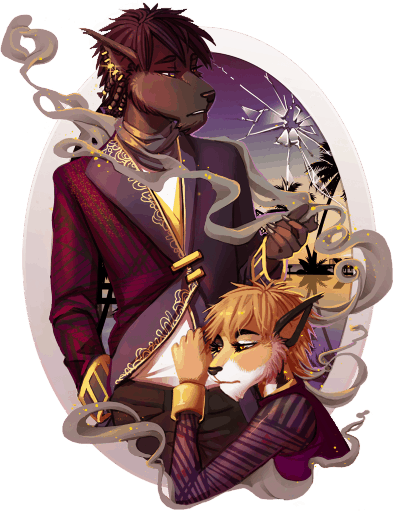
\includegraphics[width=5cm]{img/personnages/races/bothan.png}
\end{samepage}

Les Bothans sont des humanoïdes trappus, dont le corps est recouvert d'une épaisse fourrure pouvant varier du blanc-cassé à brun très foncé.
Le peuple bothan est originaire de la planète Bothawui, un monde cosmopolite épargné des troubles de la Guerre Civile Galactique en raison de la neutralité officielle du gouvernement bothan. Plusieurs colonies ont également été construites sur des planètes proches, telles que Kothlis, qui est désormais le siège d'une importante communauté. Toutes ces colonies forment l'Espace Bothan.\\
La structure sociale des Bothans est constituée par des clans familiaux, dont le nom est inclus dans le nom de chaque Bothan, à la suite d'une apostrophe.

\begin{description}[align=left]
\item [Agilité du Félin] 			% CAP +2
		Les Bothans possède la grace de leur ancêtres félins.\\
		\emph{Commence avec d6 Agi}
\item [Service de renseignement] 	% CAP +1
		Depuis plus de 300 ans ces êtres intelligents et rusés ont perfectionné leurs façons de faire, et ont développé un vaste réseau d'espions et d'informateurs destiné à recueillir toutes sortes d'informations sur les sujets les plus importants.\\
		\emph{d6 en Réseaux}
\item [Comme en plein jour] 		% CAP +1
		Grace à leur yeux de félins, les Bothans voient parfaitemnet dans l'obscurité.\\
		\emph{Vision Nocture}
\item [Déplacement rapide] 			% CAP +2
		Les Bothans, s'ils se baissent sur leur quatres pattes peuvent atteindre des vitesses de 80km/h.\\
		\emph{All = 10}
\item [Frêle] 						% CAP -2
		De contitution moins résistante, les Bothans sont moins adapté aux combats rapproché.\\
		\emph{-1 Résistance}
\item [Mauvaise réputation] 		% CAP -1
		Les ruses conduites par ce peuple, ainsi que l'opacité inhérente au Réseau Bothan, ne jouent pas en leur faveur. Certains leur reprochent de ne pas avoir prévu que l'Empire tendait une embuscade aux forces de l'Alliance.\\
		\emph{\'Etranger}
\item [Prudent] 					% CAP -1
		Les Bothans ne font rien à la légère, ils ne laissent nulle place au hazard et chaque décision est murrement réfléchie. Ils ne connaissent pas l'urgence.\\
		\emph{Prudent}
\end{description}
\subsubsection{Chiss}
\begin{samepage}
	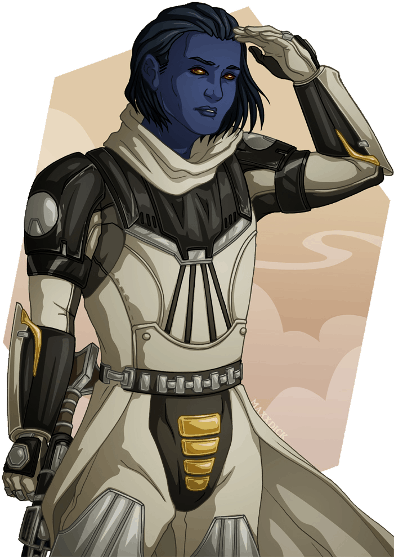
\includegraphics[width=5cm]{img/personnages/races/chiss.png}

	\vspace{-9\baselineskip}

	\begin{flushright}
		\begin{tabular}{ l l }
			\textbf{Type} 			& Humanoïde \\
		   	\textbf{Planète} 		& Csilla \\
		   	\textbf{Language} 		& Cheunh \\
		   	\textbf{Orientation} 	& Obscur \\
		\end{tabular}
	\end{flushright}
	\vspace{4\baselineskip}
\end{samepage}

Les Chiss font en moyenne 1,80m et ont une morphologie humaine. Cependant, il est impossible de les confondre à cause de leur peau bleue et de leurs yeux d’un rouge éclatant. Ils ont toujours des cheveux noirs, bien qu’avec les années, certains voient des cheveux blancs apparaitre. \\ 

La société Chiss est très évoluée. Ils ont de l’intérêt pour les arts et la science et maintiennent une puissante force militaire. Ils ont la réputation d’être de fins stratèges militaires mais leur façon de penser se retrouve dans tous les domaines de la vie quotidienne. Ils réfléchissent et pensent à différents points de vue et aux alternatives lorsqu’ils doivent prendre une décision.  

\begin{description}[align=left]
\item [Charismatique] 			% CAP +2 +2 +1
		Les Chiss sont des êtres charismatique habitué à commander des armées.\\
		\emph{+2 Cha}\\
		\emph{Commandement}\\
		\emph{d6 Connaissance (Combats)}
\item [Aquité visuelle] 		% CAP +1
		Les modifications qu’ont subies leurs yeux leur ont également donné une plus grande acuité visuelle.\\
		\emph{d6 Perception}
\item [Arrogant] 				% CAP -2
		Les Chiss sont fréquemment perçus par le reste de la galaxie, comme un peuple arrogant, calculateur et distant.\\
		\emph{Arrogant}
\item [Insensible à la Force] 		% CAP -1
		Les Chiss ne sont pas connus pour être une espèce sensible à la Force. Ils n’ont eut qu’un seul exemple d’individu sensible, en la personne de Sev’rance Tann. Cette dernière avait optée pour le côté obscur.\\
		\emph{A la création, l'augmentation de l'\^Ame coute 2pt}
\end{description}
\subsubsection{Droïde}
\begin{samepage}
	\vspace{4\baselineskip}
	\begin{tabular}{ l l }
		\textbf{Type} 			& Artificiel \\
	   	\textbf{Planète} 		& Multiple \\
	   	\textbf{Language} 		& Binaire \\
	   	\textbf{Orientation} 	& Neutre \\
	\end{tabular}

	\vspace{-11\baselineskip}

	\begin{flushright}
		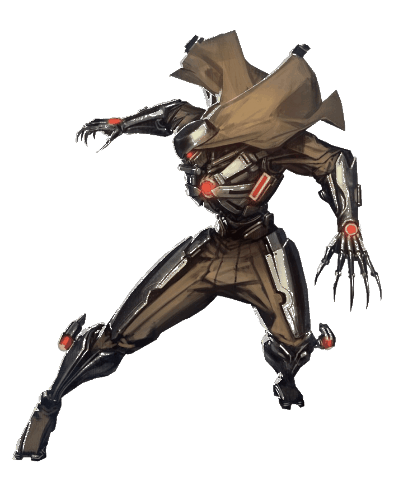
\includegraphics[width=6cm]{img/personnages/races/droide.png}
	\end{flushright}
	\vspace{-2\baselineskip}
\end{samepage}

Les Droïdes ne sont pas une race à proprement parlé mais des entités artificielles créés par d'autres races. Il peuvent être de Combat, de Protocole, de Compagnie, \ldots 
De par leur nature artificielle les Droïdes ne peuvent et ne pourront jamais utiliser la Force, c'est une notion qui leur est totalement étrangère.

\begin{description}[align=left]
\item [Créature artificielle] 	% CAP +2
		Les droides ne ressentent pas la douleur de blessures ou de la perte d'un membre.\\
		\emph{+2 pour se remettre d'un état secoué}\\
		\emph{Pas de bonus aux attaques ciblées}\\
		\emph{Pas de malus de blessure}
\item [Immunisé] 				% CAP +1
		Les maladies et les poisons sont sans effet sur les droides.\\
		\emph{Immunisé}
\item [Ambidextre] 				% CAP +2
		Un droïde ne fait pas de différence entre un membre et un autre, il peut utiliser n'importe lequel indistinctement.\\
		\emph{Ambidextre}
\item [Manque pas d'air] 		% CAP +2
		Les droïdes n'ont pas besoin de respirer, il peuvent stationné dans des lieux dépourvu d'atmosphère. Ils restent cependant sensible à la température.\\
		\emph{Ambidextre}
\item [Pas d'\^Ame] 			% CAP -3
		Il est impossible pour un droïde d'utiliser la force.\\
		\emph{\^Ame <= d6}
		\emph{Compétence Force interdite}
\item [Outsider] 				% CAP -2
		Le droïdes sont considéré comme des servants par les autres espèces, ils n'ont pas de droits et ne sont pas considéré comme faisant parti de la société.\\
		\emph{\'Etrangé}
\end{description}
\subsubsection{Gungan}
\begin{samepage}
	\vspace{-1\baselineskip}
	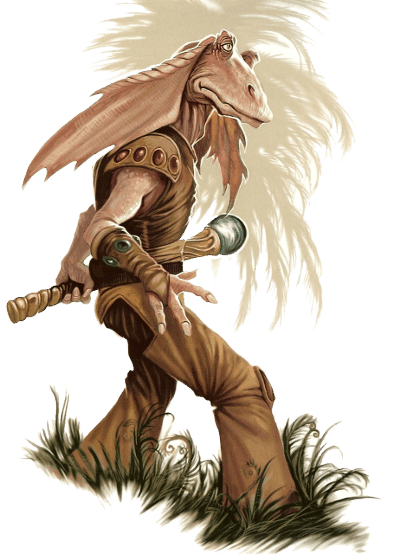
\includegraphics[width=6cm]{img/personnages/races/gungan.png}
	\vspace{-12\baselineskip}

	\begin{flushright}
		\begin{tabular}{ l l }
			\textbf{Type} 			& Amphibien \\
		   	\textbf{Planète} 		& Naboo \\
		   	\textbf{Language} 		& Gunganese \\
		   	\textbf{Orientation} 	& Lumineux \\
		\end{tabular}
	\end{flushright}

	\vspace{7\baselineskip}
\end{samepage}

Natifs de la planète Naboo, les Gungans vivent dans des cités sous-marines, évitant autant qu’ils le peuvent la race peuplant la surface : les Humains de Naboo. 

La physiologie d’un Gungan est de type humanoïde, quoique plus grand et plus fin qu’un Humain. Les Gungans possèdent de longues oreilles tombantes, des narines souples et des membranes rétractiles protégeant les yeux lors de leur déplacement aquatique. Leurs articulations sont libres et les ligaments très souples, permettant aux amphibiens de nager avec aisance sous l’eau.

La culture Gungan est une relation poussée entre la nature et l’individu. Ils essaient de ne pas utiliser la technologie.

\begin{description}[align=left]
\item [Aquatique] 			% CAP +2 +1
		Les gungans vivent dans les grandes étendues d’eau de Naboo, ils ne peuvent se noyer. Ils se déplace sous l’eau beacoup plus vite que n’importe qu’elle autre espèce.\\
		\emph{d6 Natation}\\
		\emph{Allure sous l’eau = d Natation}
		
\item [Mollusque] 			% CAP +3
		Leurs articulations sont libres et les ligaments très souples, permettant aux amphibiens de nager avec aisance sous l’eau. Cette souplesse leur permet de se faufiler dans des endroits étroits et d’esquiver les attaques avec plus de réussite.\\
		\emph{Esquive}
\end{description}
\subsubsection{Miraluka}
\begin{samepage}
	\vspace{-2\baselineskip}
	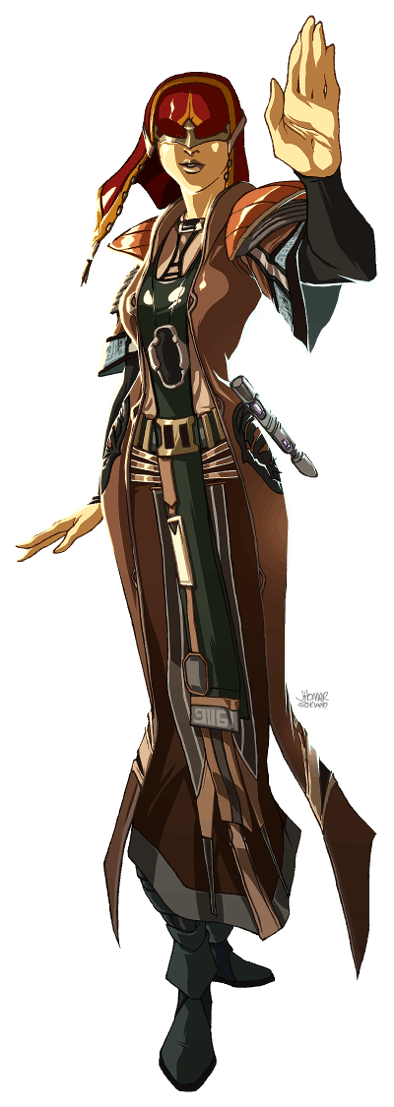
\includegraphics[width=4.5cm]{img/personnages/races/miraluka.png}

	\vspace{-5\baselineskip}

	\begin{flushright}
		\begin{tabular}{ l l }
			\textbf{Type} 			& Humanoïde \\
		   	\textbf{Planète} 		& Alpheridies \\
		   	\textbf{Langage} 		& Miralukese \\
		   	\textbf{Orientation} 	& Lumineux \\
		\end{tabular}
	\end{flushright}
\end{samepage}

Les Miraluka ressemblent beaucoup aux Humains mis à part le fait que leurs cavités oculaires sont vides et qu’ils sont capables de voir à travers la Force. A l’origine, les pacifiques Miraluka vivaient sur un monde dont le nom n’est pas passé à la postérité et qui entra dans une phase d’instabilité géophysique et géo-chimique durant laquelle l’atmosphère de la planète commença à s’évacuer dans l’espace. Des éclaireurs miraluka partirent à la recherche d’un monde où pourrait s’installer leur peuple et trouvèrent une planète habitable dans le système d’Abron : Alpheridies. 

Les Miraluka ont également tendance à masquer le haut de leur visage avec des viseurs ou des morceaux de tissus pour dissimuler leurs orbites vides, en particulier lorsqu’ils voyagent, pour ne pas attirer l’attention.


\begin{description}[align=left]
\item [Sensibilité raciale à la force] 	% CAP +2
		Il est extrêmement rare qu’une espèce toute entière soit sensible aux flux de la Force et il n’est guère étonnant que certains Miraluka, parmi ceux qui maîtrisaient le mieux la Force, aient rejoint l’Ordre Jedi.\\
		\emph{d6 \^Ame}

\item [Vision de force] 			% CAP +2 +2
		Ils perçoivent leur environnement grâce à la Force. Cette « vision » est si puissante que s’ils « regardent » un Jedi ou un Sith à travers elle, ils verront les radiations de Force qu’ils dégagent. Il faut néanmoins noter que la connexion à la Force varie en fonction de chaque Miraluka.\\
		\emph{d6 compétence Force}\\
		\emph{Pouvoir (Vision de Force) permanent et gratuit}

\item [Aveugle dans la lumière] 	% CAP -2 -2
		Du fait qu’ils n’aient pas de globe oculaire, les Miraluka voient par la force, tout ce qui n’est pas lié à la Force leur échappe. Les droïdes, par exemple, étant des "vides de Force" ne leur apparaissent pas. Il leur est impossible de lire.\\
		\emph{Handicap (Aveugle)}\\
		\emph{-1 Parade}
\end{description}
\subsubsection{Togruta}
\begin{samepage}
	\begin{tabular}{ l l }
		\textbf{Type} 			& Humanoïde \\
	   	\textbf{Planète} 		& Shili \\
	   	\textbf{Language} 		& Togru \\
	   	\textbf{Orientation} 	& Lumineux \\
	\end{tabular}

	\vspace{-9\baselineskip}
	\begin{flushright}
		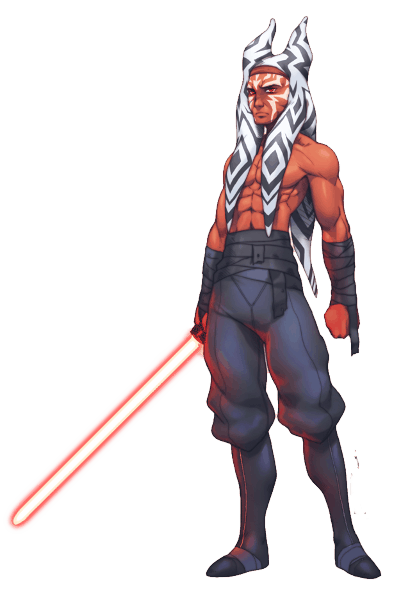
\includegraphics[width=7cm]{img/personnages/races/togruta.png}
	\end{flushright}

	\vspace{-2\baselineskip}
\end{samepage}

Les Togrutas sont des humanoïdes dont l'apparence induit souvent en erreur les observateurs peu attentifs et les fait passer pour des Twi'leks. Ils possèdent une couleur de peau rouge vif, de la même manière là encore que certaines sous-espèces de Twi-leks. Leurs yeux sont entourés d'un grand cercle blanc, et leurs montrals sont également de cette couleur. Enfin leurs lekkus sont bariolés, de manière à assurer un camouflage efficace. Le Togruta adulte atteint en général une taille moyenne de 180 cm. 


\begin{description}[align=left]
\item [Agilité] 				% CAP +2
		Les Togrutas sont des être particulièrement agile.\\
		\emph{d6 \^Agi}
\item [Montrals] 				% CAP +1 +2
		Les montrals des Togrutas renferment de puissants organes sensoriels qui réagissent aux ultrasons. En pratique cela leur permet de se repérer dans leur environnement de manière efficace et autonome, ainsi que de détecter la présence d'éventuels prédateurs sur leur monde natal, Shili..\\
		\emph{d6 Perception}\\
		\emph{Sixieme Sens}
\item [Predateur né] 			% CAP +1
		Les Togrutas sur leur planète d'origine sont des prédateurs habitué à chasser. Ils aiment leur proies fraiche.\\
		\emph{d6 Discrétion}
\item [Mauvaise réputation] 	% CAP -1
		Leur réputation n'est pas toujours excellente car des rumeurs anciennes prétendent que les Togrutas sont capables d'injecter un poison mortel à leur victime, ce qui incite évidemment à la méfiance.\\
		\emph{\'Etranger}
\item [Frèle] 					% CAP -2
		Les Togrutas sont de corpulence élancé et sont moins résistant que d'autres races.\\
		\emph{-1 Résistance}
\item [Un pour tous] 			% CAP -1
		Les Togrutas sont une espèce très loyale envers leur compagnons d'aventure, en laisser un dans l'embarras alors qu'il y avait une chance même minime de le sauver est impensable.\\
		\emph{Loyal}
\end{description}
\subsubsection{Twi'Lek}
\begin{samepage}
	\vspace{-1\baselineskip}
	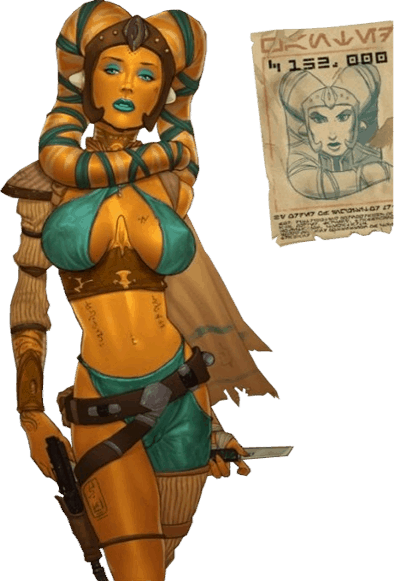
\includegraphics[width=6cm]{img/personnages/races/twilek.png}
	\vspace{-5\baselineskip}
	\begin{flushright}
		\begin{tabular}{ l l }
			\textbf{Type} 			& Humanoïde \\
		   	\textbf{Planète} 		& Ryloth \\
		   	\textbf{Language} 		& Ryl \\
		   	\textbf{Orientation} 	& Neutre \\
		\end{tabular}
	\end{flushright}
\end{samepage}

Les Twi'leks sont de grands humanoïdes, dont la peau très pigmentée peut avoir différentes couleurs selon les individus : rouge, jaune ou encore bleue par exemple. Leur trait le plus caractéristique est la paire de tentacules, appelés "lekkus", qui prend sa base au sommet de leur crâne.

Les Twi'leks utilisent leurs lekkus quand ils parlent leur langage d'origine, le twi'leki. Il s'agit d'un langage combinant communication orale et gestes, les mots étant accompagnés et complétés par les mouvements des lekkus.

La société twi'lek est divisée en deux castes très distinctes : les marchands et les guerriers.

% Les Twi'leks sont une race spéciale puisque c'est la seule à proposer des capacités différente pour les mâles et pour les femelles de la race. Attention toutefois à ce que les deux restent équilibré et à ne pas dépasser les +2 de capacité sans quoi les mâles et les femelles seraient trop différents.
\begin{description}[align=left]
\item [Rusé \& Astucieux] 			% CAP +2
		Les Twi'leks n'ont jamais eu la vie facile, entre leur monde natal pas vraiment amical et les hordes de criminels qui en veulent à leur Ryll, il leur a fallu faire preuve d'astuce pour composer avec tout cela.\\
		\emph{d6 Int}
\item [Ni chaud ni froid] 			% CAP +2
		Ryloth la terre natale des Twi'leks est composé de deux faces, l'une en permanence au soleil, à près de 300° et l'autre en permance dans l'obscurité. Le tout parcouru par de violentes tempêtes. Des conditions qui font des natifs des êtres particulièrement résistants à leur environnement.\\
		\emph{+4 pour résister aux effets négatifs de l’environnement}
\item [Lekkus Speaking] 			% Gratuit
		En plus du Ryl, les Twi'leks, grâce à leur lekkus sont capable de parler le twi'leki, ce qui s'avère difficile pour les autres races.\\
		\emph{Connaissance (twi'leki)}
\item [Belle plante (Femelles)] 	% CAP +2
		Toutes les femelles Twi'lek sont belle, au point que leur propre mâle les vendent aux pirates et autres criminels de passage pour arrondir les fins de mois.\\
		\emph{Séduisant (Cette capacité ne s'applique qu'aux personnages de sexe féminin)}
\item [Immunisé (Mâles)] 			% CAP +2
		Physiologiquement, les Twi'leks sont capables de résister à certaines toxines et maladies.\\
		\emph{Guérison rapide (Cette capacité ne s'applique qu'aux personnages de sexe masculin)}
\item [Frêles] 						% CAP -2
		Les Twi'leks sont de constitution moins résistance que les autres races.\\
		\emph{-1 Résistance}
\item [Prudent] 					% CAP -1
		Les Twi'leks en êtres intelligent prennent le temps de la réflexion et ne font pas les choses sans y réfléchir avant.\\
		\emph{Prudent}
\item [Hutt(er)] 					% CAP -1
		Les problèmes liés au commerce du Ryll ont obligé les Twi'lek à vendre leurs femmes pour présever leur monde des criminels. Les Hutt sont les premiers client de ce traffic et les Twi'leks libre ont du mal à garder leur calme face à un Hutt.\\
		\emph{Ennemi Racial (Hutt)}
\end{description}
\subsubsection{Wookie}
\begin{samepage}
	\begin{flushright}
		\begin{tabular}{ l l }
			\textbf{Type} 			& Bipèdes \\
		   	\textbf{Planète} 		& Kashyyyk \\
		   	\textbf{Language} 		& Shyriiwook \\
		   	\textbf{Orientation} 	& Lumineux \\
		\end{tabular}
	\end{flushright}
	\vspace{-6\baselineskip}
	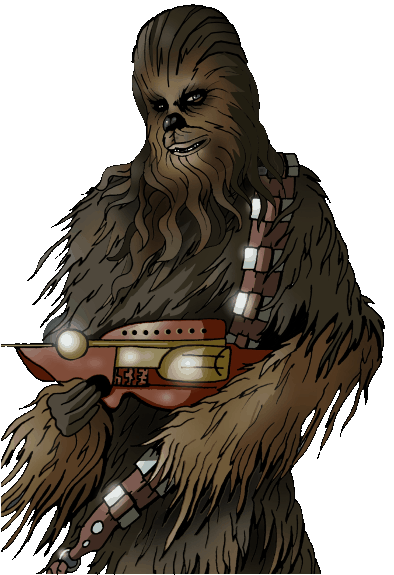
\includegraphics[width=6cm]{img/personnages/races/wookie.png}
\end{samepage}

Les Wookies sont de grand bipèdes à fourrure dépassant couramment les deux mètres de haut. Ils sont originaires de la planète Kashyyyk et n'ont que très peu de communautés en dehors de leur monde natal. Capables de vivre plusieurs siècles, les Wookies sont également dotés de longues griffes rétractiles, qu'ils utilisent principalement pour s'accrocher à la végétation dense de Kashyyyk. Leur honneur leur interdit cependant formellement d'utiliser ces griffes comme armes lors d'un combat.

\begin{description}[align=left]
\item [Force de la nature] 				% CAP +2
	L'imagerie populaire veut que les Wookies soit physiquement la race la plus forte de la galaxie (en tous cas, par rapport à sa taille).\\
	\emph{d6 For}
\item [Increvable] 						% CAP +2 +3
	Les Wookies possèdent, entres autres, de remarquables capacités de récupération, et sont capables de survivre à des blessures très graves.\\
	\emph{Increvable}\\
	\emph{Combatif}
\item [Shyriiwook] 						% CAP -1
		Les Wookies parlent entre eux leur langage, le Shyriiwook, un dialecte très complexe, en raison du mélange de feulements, rugissements, gestes et autres bruits nécessaires à son usage.\\
		\emph{Ne parle pas le Basic}
\item [Force \& Honneur] 				% CAP -2
	Comme de nombreux peuples mettant en avant des valeurs comme l'honneur, les Wookies pratiquent les serments et la "dette de vie". Celle-ci peut les amener à défendre jusqu'à la mort un étranger (même d'une autre race) auquel ils pensent devoir une grande faveur. Une dette de vie est définitive et rien ne peut la lever.\\
	\emph{Code d'honneur}
\item [Ennemis jurés] 					% CAP -1
	Les ennemis jurés des Wookies, les Trandoshans, se firent à cette époque un malin plaisir à chasser et à capturer les wookies.\\
	\emph{Ennemi Racial (Trandoshans) -4 Cha}
\item [Il faut partir à point] 			% CAP -1
	De par leur stature, les Wookies ne sont pas les êtres les plus vif de la galaxy.\\
	\emph{Allure 5}
\end{description}
\subsubsection{Zabrak}
\begin{samepage}
	\begin{flushright}
		\begin{tabular}{ l l }
			\textbf{Type} 			& Humanoïde \\
		   	\textbf{Planète} 		& Iridonia \\
		   	\textbf{Langage} 		& Zabraki \\
		   	\textbf{Orientation} 	& Obscur \\
		\end{tabular}
	\end{flushright}
	\vspace{-6\baselineskip}
	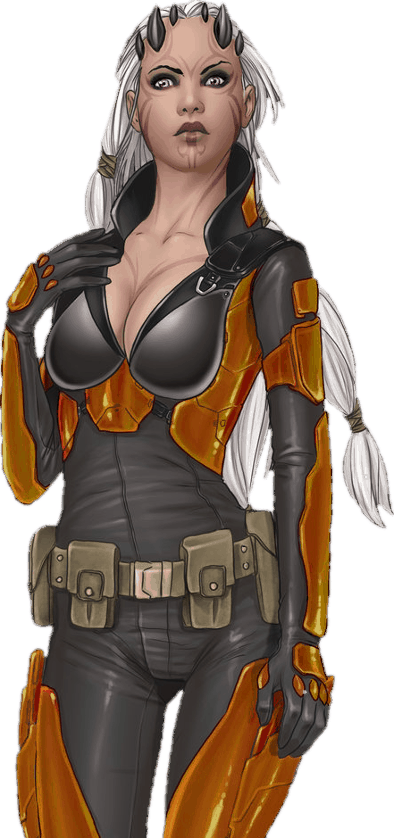
\includegraphics[width=5cm]{img/personnages/races/zabrak.png}
\end{samepage}

Originaires de la planète Iridonia, les Zabraks sont des humanoïdes d’une taille pouvant aller de 1,60 mètre à 2,10 mètres, et dont la tête était recouverte de petites cornes et le corps de tatouages, qui donnent à cette espèce un aspect parfois effrayant. Très tôt dans l’histoire galactique les Zabraks ont atteint un niveau de technologie élevé et ont pu coloniser plusieurs mondes extérieurs aux alentours de leur planète natale. On estime que cette espèce a ainsi établi huit colonies dans la Bordure Extérieure, et que les différents groupes coloniaux ont pu prospérer de façon suffisamment importante pour que les Zabraks s’identifient eux-même selon les colonies d’où ils viennent, plutôt que par rapport à Iridonia uniquement.

\begin{description}[align=left]
	\item [Endurance] 				% CAP +2
		Très tôt dans l’histoire galactique les Zabraks ont atteint un niveau de technologie élevé et ont pu coloniser plusieurs mondes extérieurs aux alentours de leur planète natale. Cette vague de colonisation à forcé l’espèce à s’adapter et à se renforcer.\\
		\emph{d6 Vig}

	\item [Braveheart] 				% CAP +2 +1
		Les Zabraks sont des explorateurs courageux et des guerriers que rien n’effraie.\\
		\emph{Atout (Brave)}\\
		\emph{d6 Combat}

	\item [Survivor] 				% CAP +1
		Les Zabraks présentent un instinct de survie supérieur à la plupart des autres espèces.\\
		\emph{d6 Survie}

	\item [Fierté mal placé] 				% CAP -2 -2
		Les Zabraks dans leur ensemble possèdent un fort caractère et une volonté de fer.\\
		\emph{Handicap (Présomptueux)}
		\emph{Handicap (Arrogant)}
\end{description}

%\subsection{Races Non Jouables}
%\input{chapitres/personnages/races/hutt}
%\input{chapitres/personnages/races/jawa}
\newpage

\subsection{Compétences}
Vous trouverez ici les Compétences utilisables\footnotemark[1] dans \swfe. L’utilisation d’une Compétence en situation normale ne devrait pas donner lieu à un jet de dé. Seules les situations de stress, lorsque le temps est compté ou que la réussite est loin d’être acquise, devraient donner lieu à un test de Compétence.

\footnotetext[1]{Seules les compétences modifiés sont détaillés ici, pour les autres sont décrite dans le bouquin de Savage Worlds.}

\begin{description}[align=left]
	\item [Combat (Agi)]
		Combat englobe toutes les attaques de corps	à corps quelle que soit l’arme de mêlée utilisée.
	\item [Conduite (Agi)]
		Conduite permet à votre héros de conduire les véhicules terrestres ou aéroglisseurs courants de l'univers Star Wars.
	\item [Connaissance (Int)]
		Connaissance est une Compétence passe-partout qu’il faut spécialiser. Elle inclue aussi les langues autre que la langue natale et le Basic.
	\item [Piratage (Int)]
		L'utilisation d'un ordinateur, la manipulation de serrure électronique ou tout autre appareil informatique est couvert par cette compétence.
	\item [Discrétion (Agi)]
		Discrétion représente la faculté de se cacher et de se déplacer en silence, mais aussi de camoufler des objets ou de subtiliser de petits objets à l’insu de tous.
	\item [Équitation (Agi)]
		Équitation permet de monter, contrôler et chevaucher tout animal domestiqué.
	\item [Escalade (For)]
		Les personnages peuvent être amenés à escalader des obstacles ou grimper une falaise pour prendre l'avantage du terrain lors d'une attaque, ou encore pour échapper à un ennemi trop coriace.
	\item [Intimidation (\^Ame)]
		Intimidation est l’art d’effrayer un adversaire par la force de sa volonté, que ce soit par une menace ouverte ou voilée ou tout simplement avec un énorme flingue.
	\item [Jeu (Int)]
		Voici un moyen rapide pour simuler une demi-heure d’une partie de jeu sans lancer les dés pour la moindre phase du jeu en question.
	\item [Lancer (Agi)]
		Lancer s’applique à toutes les armes qui se lancent, grenades, couteaux, haches, lances, etc.
	\item [Natation (Agi)]
		Natation détermine si un personnage nage ou coule comme une pierre lorsqu’il se trouve dans l’eau, ainsi que sa vitesse de déplacement en milieu aquatique.
	\item [Navigation (Int)]
		Navigation est la capacité du personnage à voyager et a se repérer dans l'espace. Il englobe aussi l'entretien journalier de l'équipement utilisé.
	\item [Perception (Int)]
		Perception représente la vigilance d’un héros et son habilité à découvrir objets ou indices.
	\item [Pilotage (Agi)]
		Pilotage permet d’utiliser tous les types d’appareils aériens ou spatiaux communs.
	\item [Pistage (Int)]
		Pistage permet de suivre les traces d’un ou de plusieurs individus sur tout type de terrain.
	\item [Recherche (Int)]
		Recherche permet d’obtenir des informations avec une bibliothèque, HoloNet, les journeaux ou toute autre source écrite.
	\item [Réparation (Int)]
		Réparation représente la capacité à remettre en état gadgets, véhicules, armes et autres machines.
	\item [Réseaux (Int)]
		Réseaux permet d’obtenir des informations dans la rue, les bars ou par des contacts en utilisant la menace, la corruption ou en offrant des verres. Cette compétence peut aussi représenté les informateurs du héro.
	\item [Sarcasme (Int)]
		Sarcasme est une attaque contre l’amour-propre d’un individu en le ridiculisant par la parole ou le geste.
	\item [Soins (Int)]
		Soins consiste à savoir comment guérir les plaies et traiter les blessures.
	\item [Survie (Int)]
		Survie permet de trouver nourriture, eau ou abri en milieu hostile.
	\item [Tir (Agi)]
		Tir concerne toute tentative pour toucher une cible avec n’importe quelle arme à distance (arc, pistolet, lance-roquettes, etc.).
\end{description}

\begin{paperbox}{Piratage}
	Cette compétence vient remplacer le Crochetage qui dans Star Wars n'a pas une grosse utilité. La compétence Piratage (Informatique) va s'utiliser de la même façon mais sur l'Inellect au lieu de de l'Agilité. L'informatique pourra être utilisé dés qu'un ordinateur entre en scène. On pourra par exemple déverrouiller des sas de vaisseau ou stoppé un signal d'alarme ou encore désactiver des capteurs à plus haut niveau.

	Les Droïde n'en sont pas systématiquement pourvu, cela dépend de leur programmation.
\end{paperbox}

\begin{paperbox}{Navigation}
	La navigation exite mais son domaine d'application change un peu, on ne parle pas dans Star Wars de bateau mais de vaisseaux spatiaux. La navigation est alors la capacité du héro à s'orienter dans le vide cidéral. Mais cela s'applique aussi au sol pour se repérer sur une carte par exemple.
\end{paperbox}

\newpage % Acts as columbreak because of twocolumn option; for pagebreak use \clearpage

% For more columns, you can say \begin{dndtable}[your options here}.
% For instance, if you wanted three columns, you could say
% \begin{dndtable}{XXX}. The usual host of tabular parameters are
% aailable as well.
\header{Nice table}
\begin{dndtable}
   	\textbf{Table head}  & \textbf{Table head} \\
   	Some value  & Some value \\
   	Some value  & Some value \\
   	Some value  & Some value
\end{dndtable}

\begin{paperbox}{Do the Players need direction?}
	\lipsum[1]
\end{paperbox}

% You can optionally not include the background by saying
% begin{monsterboxnobg}
% \begin{monsterbox}{Monster Foo}
% 	\textit{Small metasyntatic variable (golbinoid), neutral evil}\\
% 	\hline
% 	\basics[%
% 	armorclass = 12,
% 	hitpoints  = 16 (3d8 + 3),
% 	speed      = 50 ft
% 	]
% 	\hline
% 	\stats[
%     STR = \stat{12}, % This stat command will autocomplete the modifier for you
%     DEX = \stat{7}
% 	]
% 	\hline
% 	\details[%
% 	% If you want to use commas in these sections, enclose the
% 	% description in braces.
% 	% I'm so sorry.
% 	languages = {Common Lisp, Erlang},
% 	]
% 	\hline \\[1mm]
% 	\begin{monsteraction}[Monster-super-powers]
% 		This Monster has some serious superpowers!
% 	\end{monsteraction}
% 	\monstersection{Actions}
% 	\begin{monsteraction}[Generate text]
% 		This one can generate tremendous amounts of text! Though only when it wants to.
% 	\end{monsteraction}
% 
% 	\begin{monsteraction}[More actions]
%     See, here he goes again! Yet more text.
% 	\end{monsteraction}
% \end{monsterbox}
